\documentclass[a4paper,utf8]{article}
\usepackage{exemple}
\usepackage[normalem]{ulem}
\usepackage{amsfonts}
\usepackage{graphicx}
\usepackage{MnSymbol,wasysym}
\usepackage{hyperref}
\usepackage[french]{babel}
\usepackage{graphicx}

\formation{L3MI}
\date{15/01/2017}
\matiere{Conception Orient�e Objet}
\titre{Projet : Tetris Attack }

\newcommand\code[1]{\textsf{#1}}
\newcommand\srdjan[1]{{\color{red} #1}}

\begin{document}

\entete

\begin{center}
	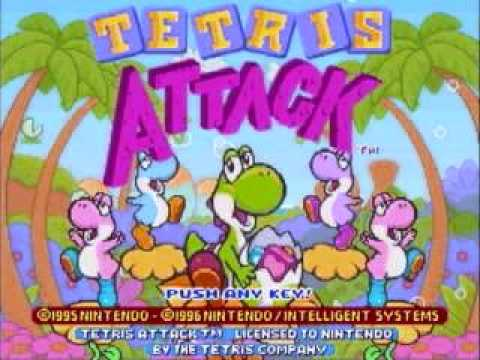
\includegraphics[scale=0.9]{img1.jpg}
\end{center}

\section{Description du Projet}
Tetris Attack est un puzzle-game � 2 joueurs sorti en 1995 sur Super Nintendo. Ce jeu est une variante du bien connu Tetris � 2 joueurs. Dans cette version, l'objectif est d'assembler des blocs entre eux afin de les faire dispara�tre avant que l'ensemble des blocs n'atteignent le haut de l'�cran. Toutefois, ici, 2 joueurs s'affrontent en parall�le et peuvent � l'aide de diff�rentes combinaisons envoyer de nouveaux blocs de briques � leur adversaire afin de pr�cipiter sa perte. Ce jeu couple � la fois, la simplicit� de Tetris � la dynamicit� n�cessaire d'un bon Versus.

\section{L'Organisation }

\subsection{L'Equipe}
\begin{itemize}
\item Vincent : jeu principal , graphique , IA. 
\item Lo�ck : jeu principal , graphique , IA.
\item Mohammed: menu , diff�rent �crans pour config , graphique.
\item K�vin: menu , diff�rent �crans pour config , graphique.
\end{itemize}

\subsection{Le Travail r�alis�}
A l'heure actuel le menu touche � sa fin principalement fait par Lo�ck qui a r�alis� toutes les animations : �cran titre, curseur, �cran de fond ainsi que les diff�rents panels.
Pour ma part (Vincent) j'ai r�alis� la s�lection des personnages pour 1 et 2 joueurs et une grille 1 joueur fonctionnelle ainsi que l'incorporation des sons dans le jeu.
Du cote de K�vin, il travaille toujours avec Mohammed sur la modification des commandes qui tra�ne malgr� mes relances toutes les semaines.

\end{document}